\documentclass[a4paper,pdftex]{article}

\usepackage{array}
\usepackage{placeins}

\usepackage{hopsantut}
\usepackage{csquotes}

\hypersetup{pdfauthor={Robert Braun}, pdftitle={Hopsan Tutorial - Running an Optimization}, pdfsubject={Hopsan Tutorial}}

\begin{document}
\maketitle{Running an Optimization}

\section*{Using the optimization dialog}
Numerical optimization is an important tool for automatically finding a desired parameter set for a model. Hopsan contains an optimization dialog from where optimizations can be controlled. This guide shows how to optimize control parameters for a simple hydraulic position servo using the Complex-RF algorithm. Optimization in Hopsan can either be performed from a dialog or by loading previously saved (or manually created) script files. This tutorial demonstrates both methods.

\begin{tutenumerate}
\tutitem{Open the model}
The \textit{Welcome} tab has a box with example models. Open the \textit{Position Servo} example model.

\FloatBarrier
\begin{figure}[h]
\center
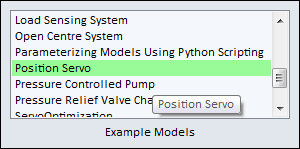
\includegraphics[width=0.5\textwidth]{gfx/optimization/openmodel.png}
\end{figure}
\FloatBarrier

This model describes of a hydraulic position servo, where a PI-controller is used to control the position. This consists of a proportional gain ($K_{p}$) and an integrator gain ($K_{i}$).  The values of these gains will decide the speed and stability of the servo. It is thus desirable to find as good controller parameters as possible.

\tutitem{Simulate}
Simulate the model by clicking the simulate icon.
 
\icon{0}{gfx/Hopsan-Simulate.png}{Simulate current project (Ctrl-Shift-S)}

Now double click on the \enquote{Scope} component on top of the model. Two curves will be plotted, the reference signal and the actual position. The reference signal is a step, and the position shows the corresponding step response. As you can see, it is quite oscillative. We want to adjust the control parameters to reduce its rise time, overshoot and settling time by using the \textit{optimization} feature.

\tutitem{Open the dialog} 
Click the optimization icon to open the dialog.

\icon{0}{gfx/Hopsan-Optimize.png}{Open optimization dialog (Ctrl-Shift-Z)}

\pagebreak

\tutitem{Optimization settings} 
The first page should look like this:

\FloatBarrier
\begin{figure}[h]
\center
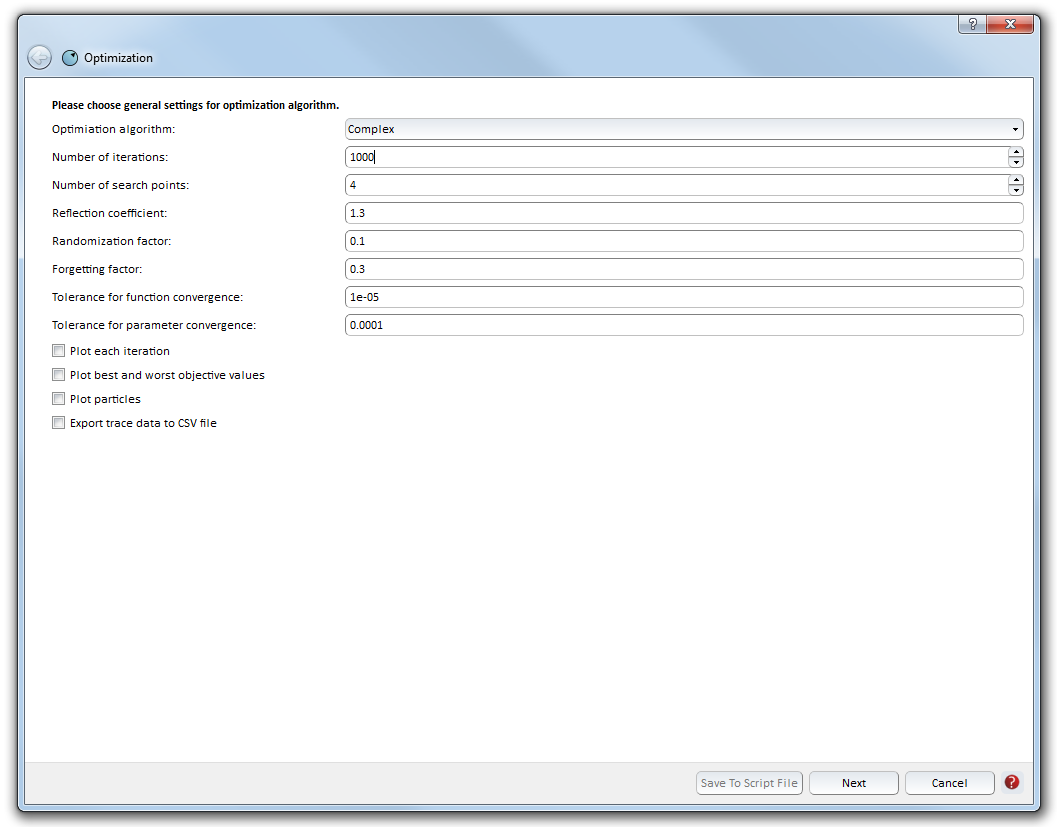
\includegraphics[width=0.7\textwidth]{gfx/optimization/screenshot-opt1.png}
\end{figure}
\FloatBarrier

From here you can choose the general settings for the optimization.
\begin{itemize}
\item Set \textit{Algorithm} to \textit{Complex}
\item Set \textit{Number of iterations} to 1000
\item Set \textit{Number of points} to 4
\end{itemize}
Leave all other settings unchanged for now.

\tutitem{Choose optimization parameters} 
Next page controls the parameters in the model that shall be optimized. 

\FloatBarrier
\begin{figure}[h]
\center
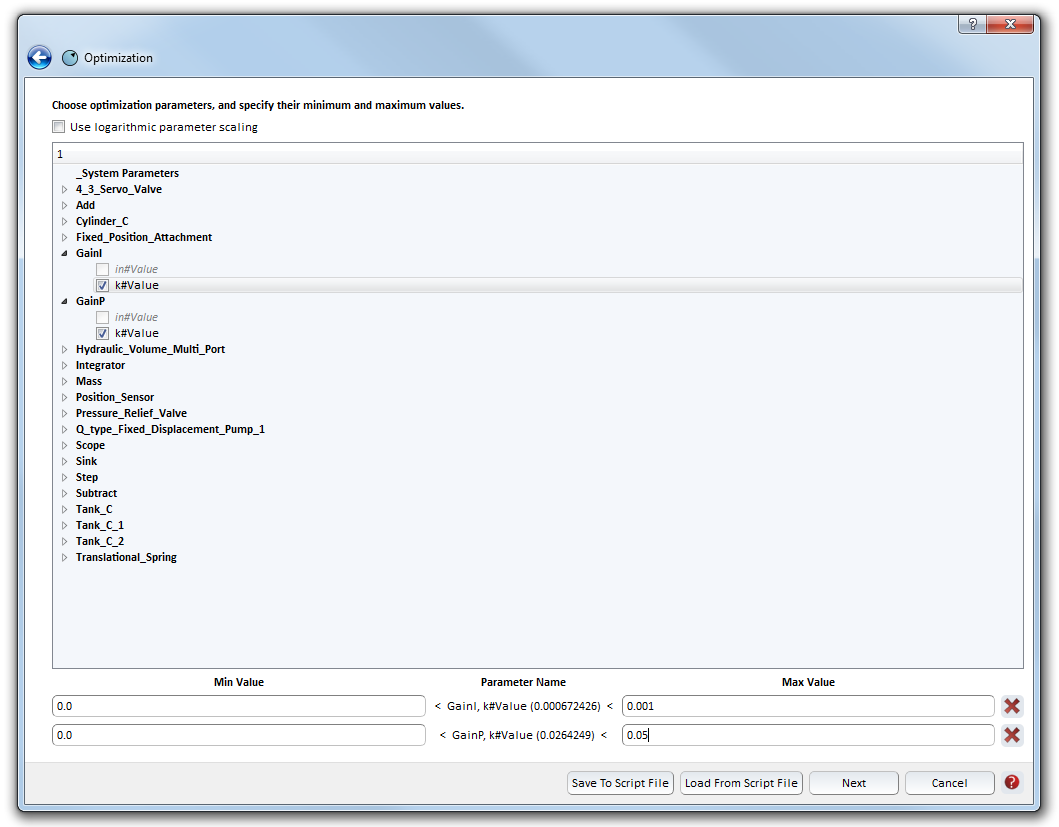
\includegraphics[width=0.7\textwidth]{gfx/optimization/screenshot-opt2.png}
\end{figure}
\FloatBarrier

Check the following parameters in the list:

\begin{itemize}
\item GainI $\rightarrow$ k\#Value
\item GainP $\rightarrow$ k\#Value
\end{itemize}

Then give them the following min and max values:

{\renewcommand{\arraystretch}{1.2} 
\begin{tabularx}{\linewidth}{X X X}
\textbf{Parameter} & \textbf{Min} & \textbf{Max} \\
\specialrule{1.3pt}{0pt}{0pt}
GainI, k\#Value & 0 & 0.001 \\
GainP, k\#Value & 0 & 0.04 \\
\end{tabularx}
}

\tutitem{Choose objective functions} 
The optimization algorithms use objective functions to calculate how good a certain point in the parameter space is. From the third page this can be chosen. In this model we want the actual position to be as close as possible to the reference signal. To do this, check the following variables in the list:
\begin{itemize}
\item{Position\_Sensor} $\rightarrow$ \textbf{out} $\rightarrow$ Value
\item{Step} $\rightarrow$ \textbf{out} $\rightarrow$ Value
\end{itemize}

Then choose \enquote{Minimize} and \enquote{Absolute Average Difference} in the boxes. Click \enquote{Add Function}.

\FloatBarrier
\begin{figure}[htb]
\center
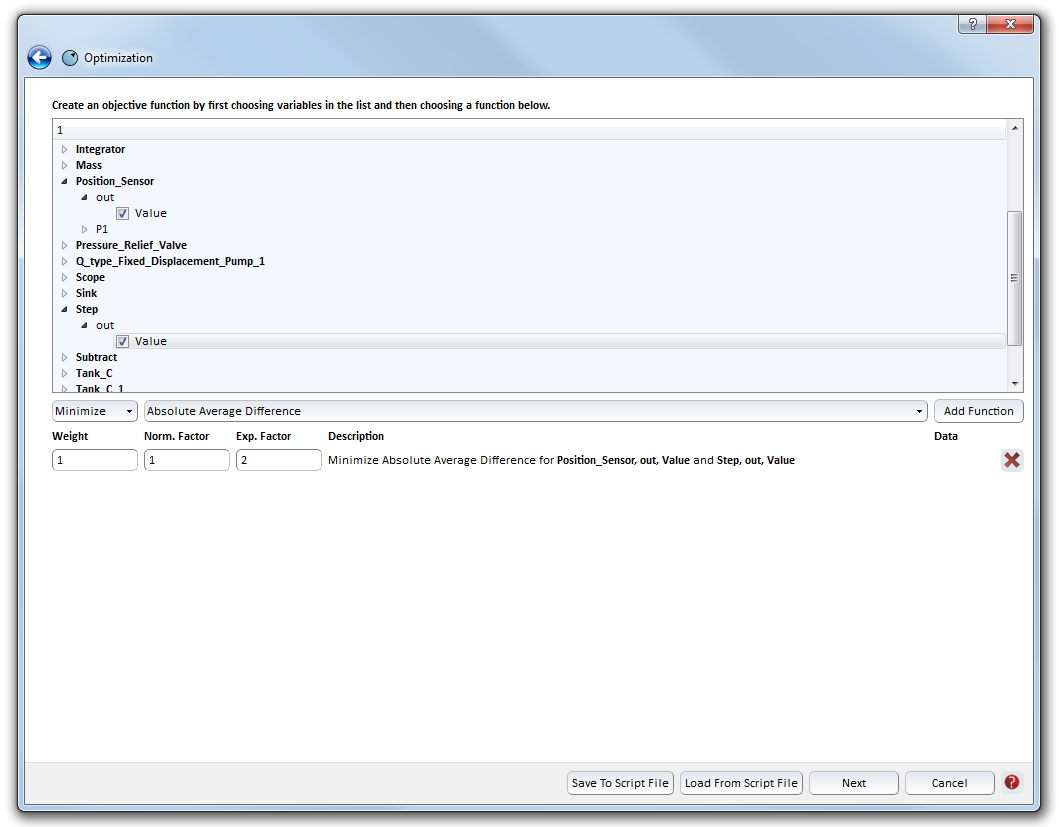
\includegraphics[width=0.7\textwidth]{gfx/optimization/screenshot-opt3a.png}
\end{figure}
\FloatBarrier

Apart from minimizing the average difference, we also want to minimize the overshoot of the step response. 
\begin{itemize}
\item Uncheck \textbf{Step} $\rightarrow$ \textbf{out} $\rightarrow$ Value
\end{itemize}

Now choose \enquote{Minimize} and \enquote{Overshoot}, and then click \enquote{Add Function}. In the box called \enquote{arg1}, change the value to 0.7. 

\newpage
Now we have added a second objective function. The total objective function will the sum of these. As they may not be equally important or equally scaled, it is possible to weight the individual functions.  Change \enquote{Weight} for the first function to 10. Now the page should look like this:

\FloatBarrier
\begin{figure}[htb]
\center
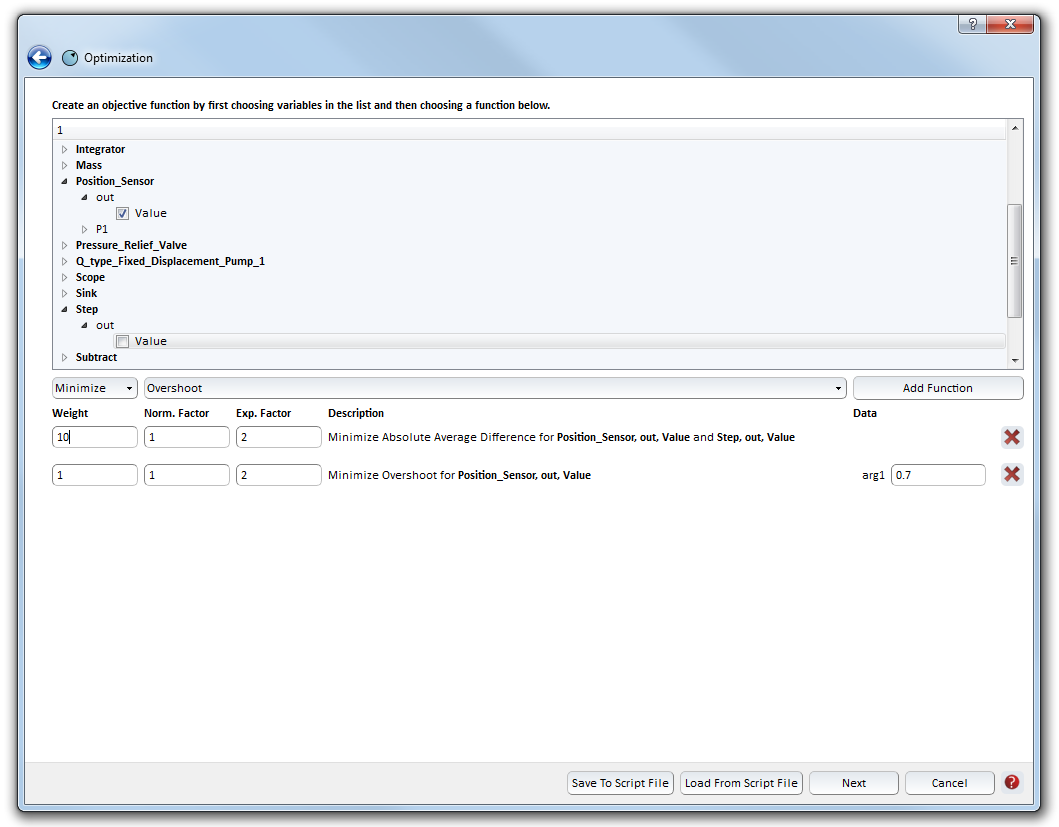
\includegraphics[width=0.7\textwidth]{gfx/optimization/screenshot-opt3b.png}
\end{figure}
\FloatBarrier

\tutitem{Start the optimization} 
Next page shows the generated script code. Modifications can be made if necessary, but leave it as it is for now.

\FloatBarrier
\begin{figure}[htb]
\center
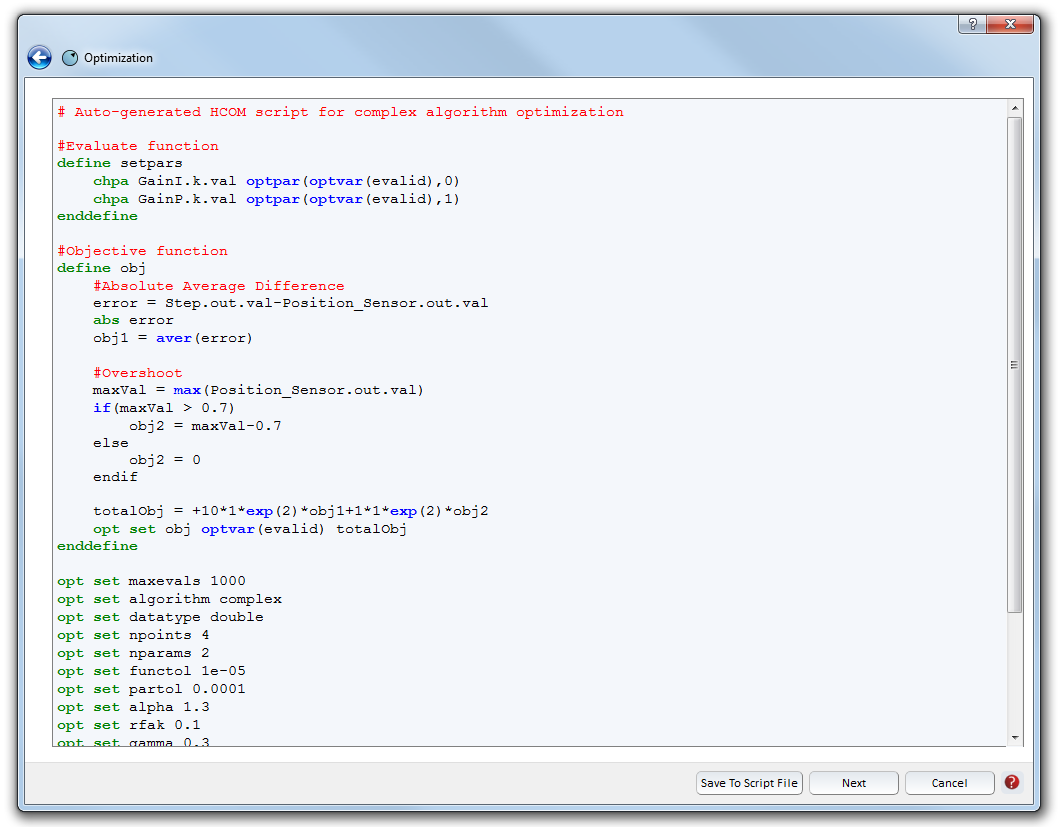
\includegraphics[width=0.7\textwidth]{gfx/optimization/screenshot-opt4.png}
\end{figure}
\FloatBarrier

\newpage
Go to the next page. From here the optimization can be executed:

\FloatBarrier
\begin{figure}[htb]
\center
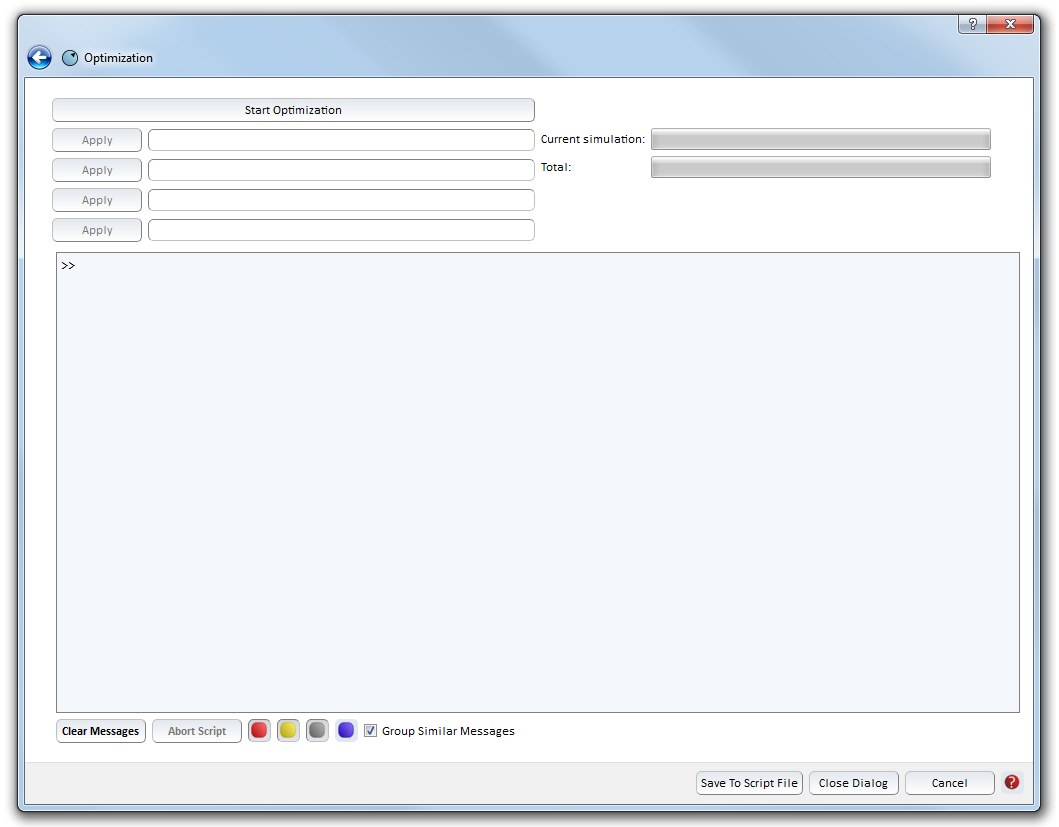
\includegraphics[width=0.7\textwidth]{gfx/optimization/screenshot-opt5a.png}
\end{figure}
\FloatBarrier

Click on \enquote{Start Optimization}. During the optimization the objective function values and the values of the optimization parameters are shown for the different points. The best point is shown in green, and the worst in red.

\FloatBarrier
\begin{figure}[htb]
\center
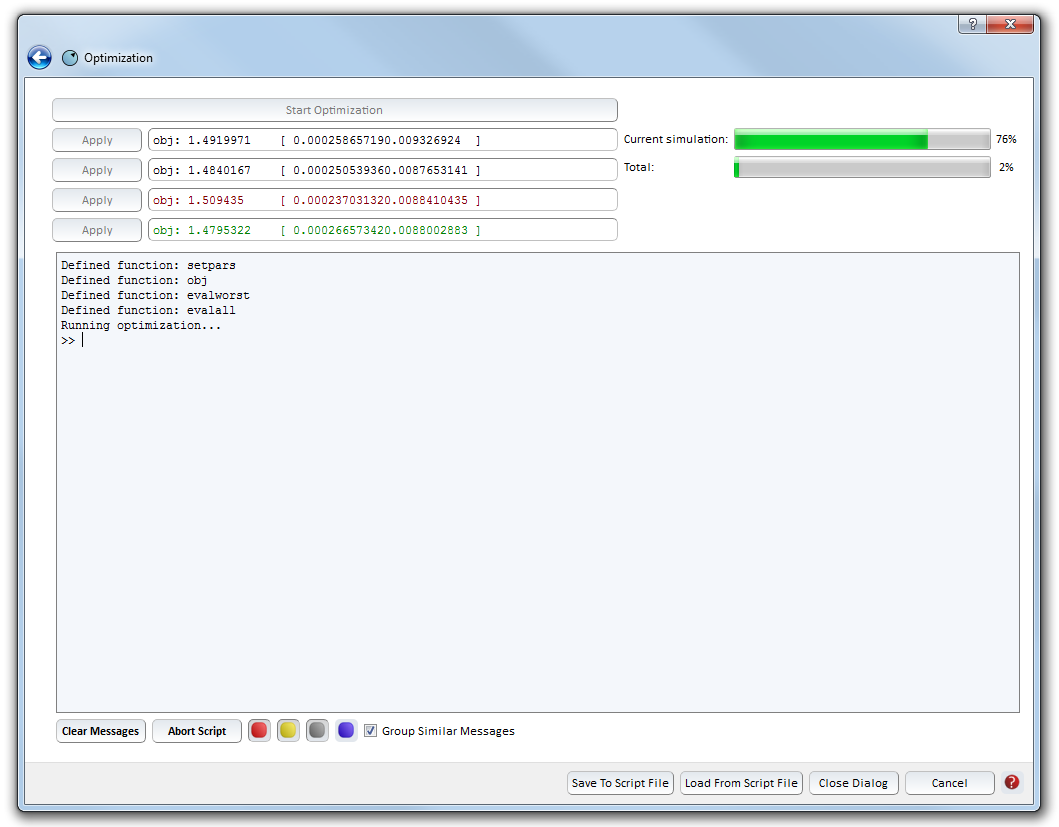
\includegraphics[width=0.7\textwidth]{gfx/optimization/screenshot-opt5b.png}
\end{figure}
\FloatBarrier

\newpage
\tutitem{Evaluate the results} 
Once the optimization has finished, we can evaluate the results. Parameters from a point can be written back to the original model by using the \enquote{Apply} buttons. 

\FloatBarrier
\begin{figure}[htb]
\center
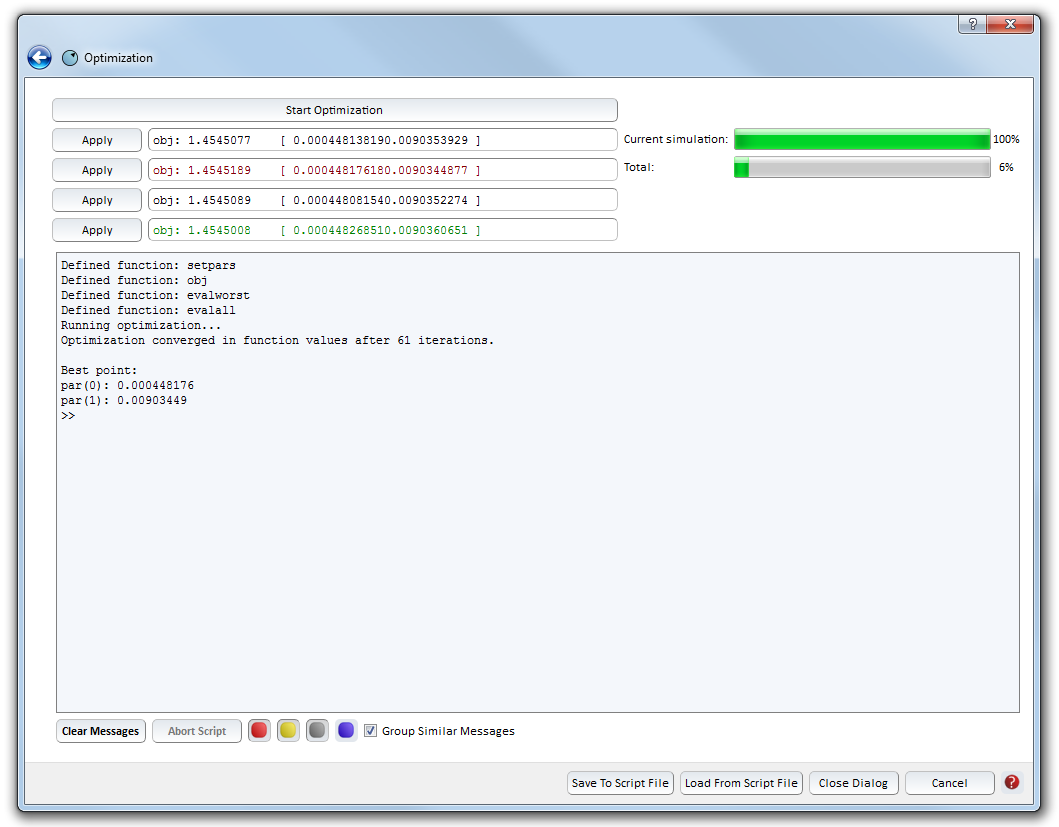
\includegraphics[width=0.7\textwidth]{gfx/optimization/screenshot-opt5c.png}
\end{figure}
\FloatBarrier

Click the \enquote{Apply} button for the point with green text (the best point). Then go back to the original model and click the Simulate button again.

\icon{0}{gfx/Hopsan-Simulate.png}{Simulate current project (Ctrl-Shift-S)}

Now plot the step response by double clicking the scope component on top of the model. If a desirable result has not been found, it can be necessary to change objective functions or parameters and re-run the optimization.

\end{tutenumerate}

\section*{Optimizing from script files}
It is often necessary to re-use the settings from the optimization more than once. This can be done by saving the optimization scripts to a file, and loading them again later.

\begin{tutenumerate}
\tutitem{Follow steps 1-7 above}\vspace{-\baselineskip}

\tutitem{Saving a script file} 
Click on Save script file in the dialog.

\tutitem{Loading a script file} 
To load a previously saved script file, click on Load script file in the dialog. You will be taken directly to the code tab. Go to the last tab and start the optimization as before. Note that the settings on the first three pages are not updated by the script. Going back to these might re-generate the script and overwrite the loaded code.

\tutitem{Loading a script file from command terminal} 
It is also possible to load a script file from the command terminal. Just write \enquote{exec} followed by the path to the file. Hopsan will automatically understand that this is an optimization script and start the dialog. You can use \enquote{pwd} to show current directory and \enquote{cd} to change directory if necessary. Example: \texttt{>{}> exec ..\textbackslash folder\textbackslash myscript.hcom}

\end{tutenumerate}

\end{document}